\subsection{章节概述}
违约概率预测模型的好坏很大程度上取决于特征工程。传统特征工程是通过不断手动尝试分箱,WOE编码,IV值筛选,特征交叉组合等方法来提取有效特征。本文提出了一种\textbf{基于自编码的特征提取方法},它在传统方法提取到的特征基础上,利用神经网络对特征进行低维空间的非线性映射和进一步压缩提取,最后将得到的全新特征作为分类模型的输入。\\

经过调查和后续的实验结果分析,该方法确实能够使得树模型的分类准确率有一定程度的提升,并且在当前风控领域并没有使用先例,属于\textbf{全新}的模型思路。\\

在特征工程方面,本章节将介绍WOE编码和IV值的基本内容,并从逻辑回归$\rightarrow$深度学习$\rightarrow$自编码器的推导关系出发,层层递进,介绍创新点的主要灵感来源。在分类模型方面,将简要介绍逻辑回归、随机森林、LightGBM和全连接深度神经网络分类器。

\subsection{WOE编码和IV值}

\subsubsection{WOE编码}
WOE的全称是“Weight of Evidence”,即证据权重。WOE是对原始自变量的一种编码形式。

要对一个变量进行WOE编码,需要首先把这个变量进行分组处理(也叫离散化、分箱等)。分组后,对于第i组,WOE的计算公式如下:

\begin{equation}
    \begin{aligned}
        WOE_i = \ln(\frac{Py_i}{Pn_i})=\ln(\frac{\frac{\sum y_i}{\sum y_T}}{\frac{\sum n_i}{\sum n_T}})
    \end{aligned}
\end{equation}

其中,$Py_i$是这个组中响应客户(风险模型中,对应的是违约客户,总之,指的是模型中预测变量取值为1的个体)占所有样本中所有响应客户的比例,$Pn_i$是这个组中未响应客户占样本中所有未响应客户的比例,$\sum y_i$是这个组中响应客户的数量,$\sum n_i$是这个组中未响应客户的数量,$\sum y_T$是样本中所有响应客户的数量,$\sum n_T$是样本中所有未响应客户的数量。\\

从这个公式中可以体会到,WOE表示的实际上是“当前分组中响应客户占所有响应客户的比例”和“当前分组中没有响应的客户占所有没有响应的客户的比例”的差异。对这个公式做一个简单变换,可以得到:

\begin{equation}
    \begin{aligned}
        WOE_i = \ln(\frac{Py_i}{Pn_i})=\ln(\frac{\frac{\sum y_i}{\sum y_T}}{\frac{\sum n_i}{\sum n_T}})=\ln(\frac{\frac{\sum y_i}{\sum n_i}}{\frac{\sum y_T}{\sum n_T}})
    \end{aligned}
\end{equation}

变换以后WOE表示的是当前这个组中响应的客户和未响应客户的比值与所有样本中该比值的差异。这个差异为两个比值的比值取对数表示。WOE越大,这种差异越大,这个分组里的样本响应(用户违约)的可能性就越大,WOE越小,差异越小,这个分组里的样本响应(用户违约)的可能性就越小。这就是WOE编码所表示的意义。

\subsubsection{IV值}

IV的全称是Information Value,中文意思是信息价值,或者信息量。在用逻辑回归、决策树等模型方法构建分类模型时,经常需要对自变量进行筛选。IV值依赖WOE编码,是一个很好的衡量自变量对目标变量影响程度的指标。\\

对于每个分组i,$IV_i$的表达式如下:

\begin{equation}
    \begin{aligned}
        IV_i & = (Py_i-Pn_i)\cdot WOE_i                                                                                  \\
             & = (Py_i - Pn_i)\cdot \ln(\frac{Py_i}{Pn_i})                                                               \\
             & =(\sum \frac{y_i}{y_T}-\sum \frac{n_i}{n_T}) \cdot \ln(\frac{\sum \frac{y_i}{y_T}}{\sum \frac{n_i}{n_T}})
    \end{aligned}
\end{equation}


将该变量各分组的IV值相加便可计算得到$IV=\sum IV_i$

\subsection{从逻辑回归到深度学习}
\subsubsection{简要说明}
逻辑回归是一种常见的分类手段,然而它对某些复杂的非线性分类场景却无能为力,深度学习可以看做是多个逻辑回归的组合,通过特征转换和降维达到非线性分类的效果。本小节将从这一观点出发,介绍从逻辑回归到深度学习的推导过程。此外,这一过程也为自编码方法的提出提供了主要灵感。

\subsubsection{逻辑回归}

假设在二元分类的场景下,$C_1$和$C_2$为两个不同的类别,则根据逻辑回归的思想,用参数$(w,b)$组合成$z$,并通过sigmoid函数缩放到0-1范围内,就得到了样本点$x$属于某一类的概率$P_{w,b}(C_i|x)$


\begin{equation}
    \begin{aligned}
        P_{w,b}(C_1|x)=\sigma(z)=\frac{1}{1+e^{-z}} \\
        z=w\cdot x+b=\sum\limits_i w_ix_i+b
    \end{aligned}
\end{equation}

\begin{figure}[H]
    \centering
    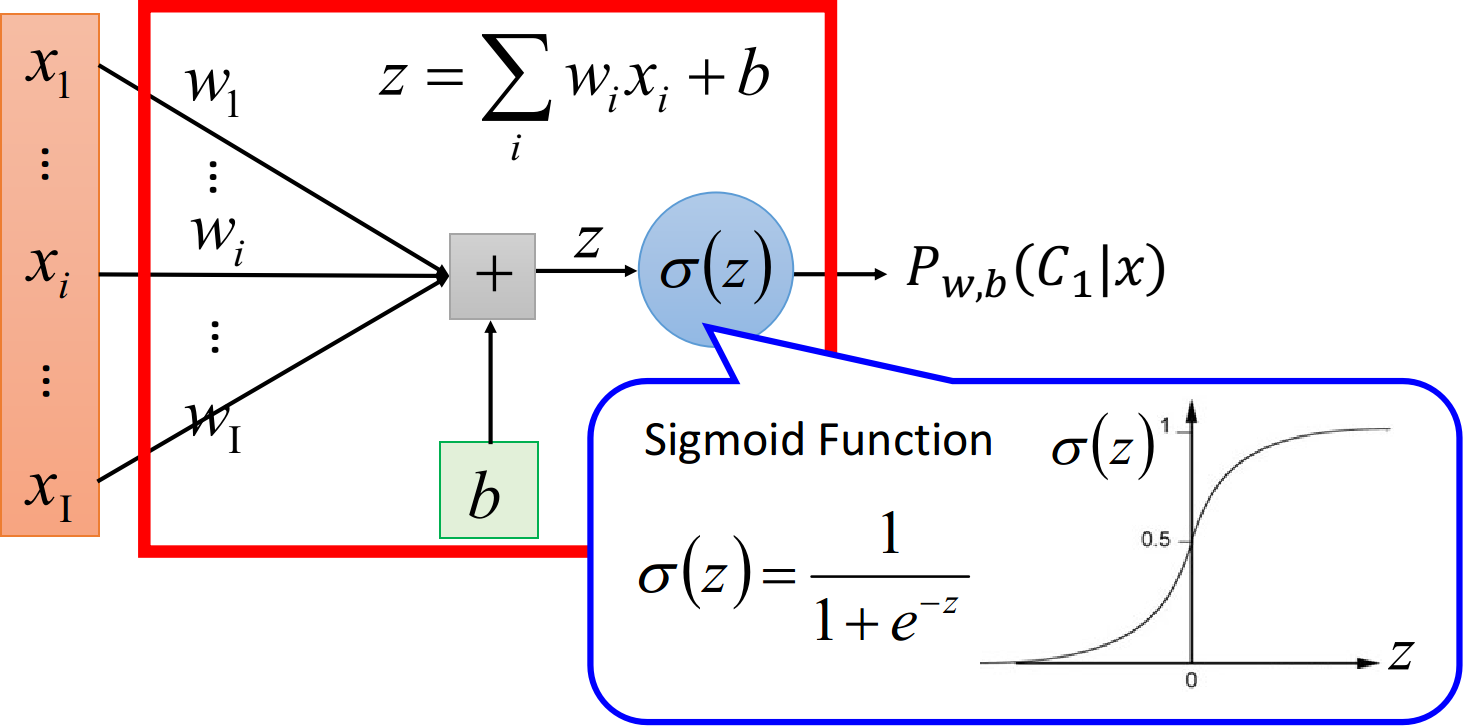
\includegraphics[width=0.5\linewidth]{LR.png}
    \caption{逻辑回归示意图}
    \label{fig:LR}
\end{figure}

假设Training data是从我们定义的Posterior Probability中产生的(后置概率,某种意义上就是概率密度函数),而w和b决定了这个Posterior Probability,此时可以去计算某一组w和b产生这N个样本点的概率,根据极大似然估计的思想,最好的那组参数就是有最大可能性产生当前N个样本点分布的$w^*$和$b^*$。最终利用极大似然估计法推导出其损失函数,并表示为交叉熵的形式如下:

\begin{equation}
    \begin{aligned}
        w^*,b^* & =\arg \max\limits_{w,b} L(w,b)                                                 \\
                & =\arg\min\limits_{w,b}(-\ln L(w,b)                                             \\
                & =\sum\limits_n -[\hat{y}^n \ln f_{w,b}(x^n)+(1-\hat{y}^n) \ln(1-f_{w,b}(x^n))]
    \end{aligned}
\end{equation}

随后计算出参数的偏导,利用梯度下降法更新参数即可:

\begin{equation}
    \begin{aligned}
        w_i=w_i-\eta \sum\limits_{n}-(\hat{y}^n-f_{w,b}(x^n))x_i^n
    \end{aligned}
\end{equation}

相比于square error, 损失函数选择cross entropy能够加快参数更新的步伐和速度,而不会导致图2中由于损失函数曲面过于平缓而停滞不前的现象

\begin{figure}[H]
    \centering
    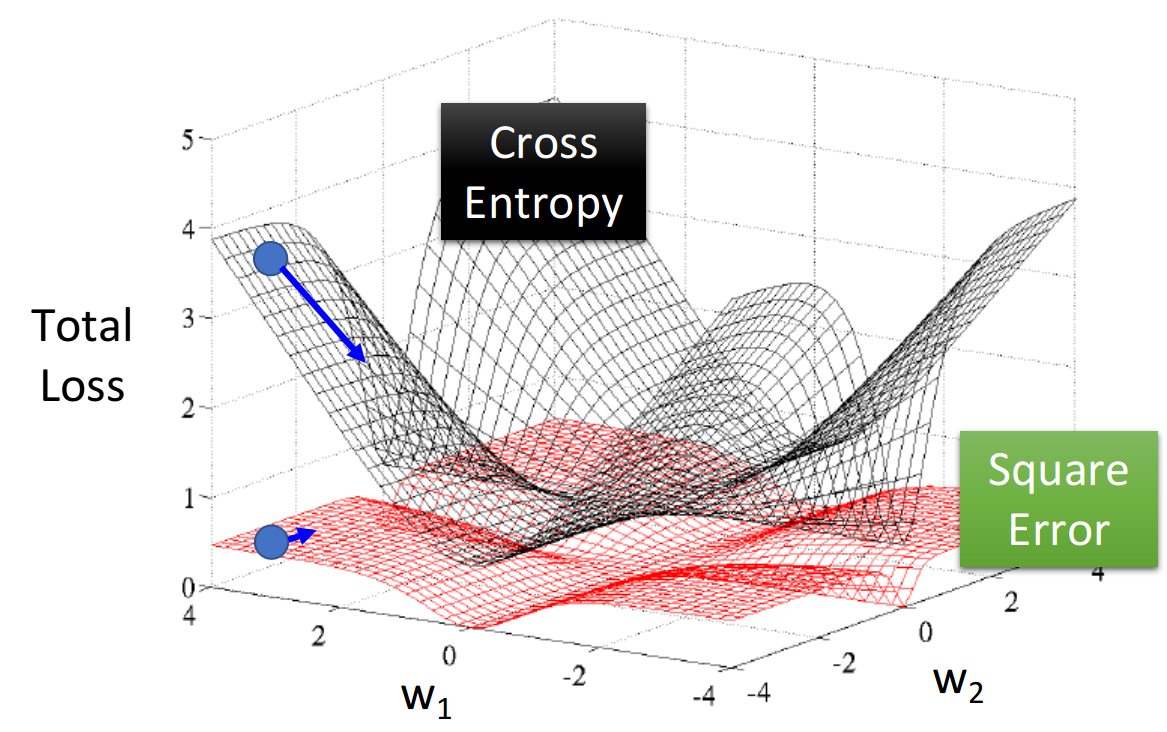
\includegraphics[width=0.5\linewidth]{ce.png}
    \caption{交叉熵vs方均根}
    \label{fig:ce}
\end{figure}

\subsubsection{逻辑回归的限制}

Logistic Regression的应用其实有不少的限制,给出图3中样本点分布,想要用逻辑回归对它进行分类,其实是做不到的。因为逻辑回归在两个class之间的boundary就是一条直线,但是在这个平面上无论怎么画直线都不可能把图中的两个class分隔开来。

\begin{figure}[H]
    \centering
    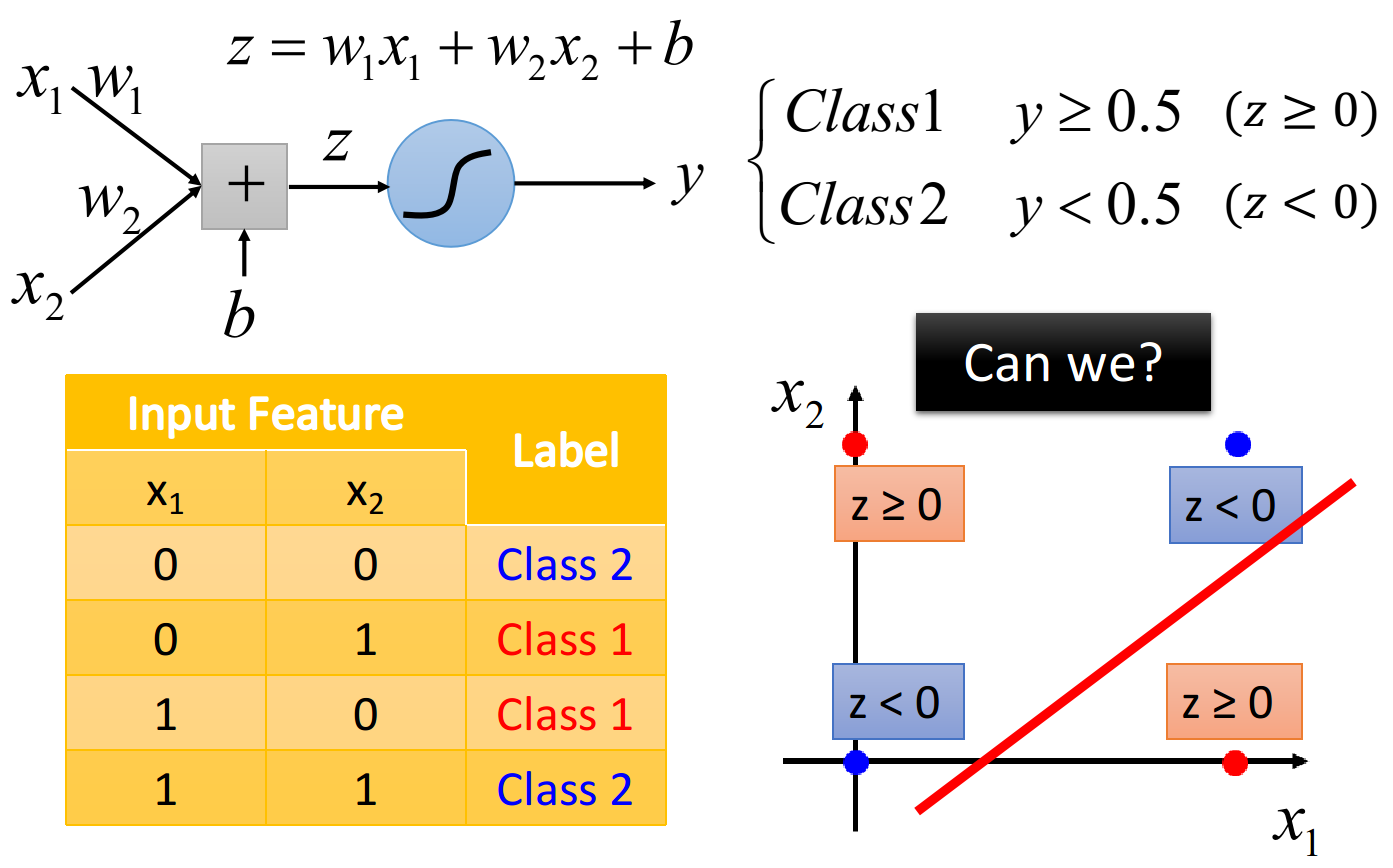
\includegraphics[width=0.6\linewidth]{limit.png}
    \caption{逻辑回归的限制}
    \label{fig:limit}
\end{figure}

如果坚持要用逻辑回归的话,可以使用Feature Transformation把原先的特征分布投影到一个比新的特征空间。\\

假设定义$x_1'$是原来的点到$\begin{bmatrix}0\\0 \end{bmatrix}$之间的距离,$x_2'$是原来的点到$\begin{bmatrix}1\\ 1 \end{bmatrix}$之间的距离,重新映射之后如图4右侧所示(红色两个点重合),此时逻辑回归就可以顺利把它们划分开来。

\begin{figure}[H]
    \centering
    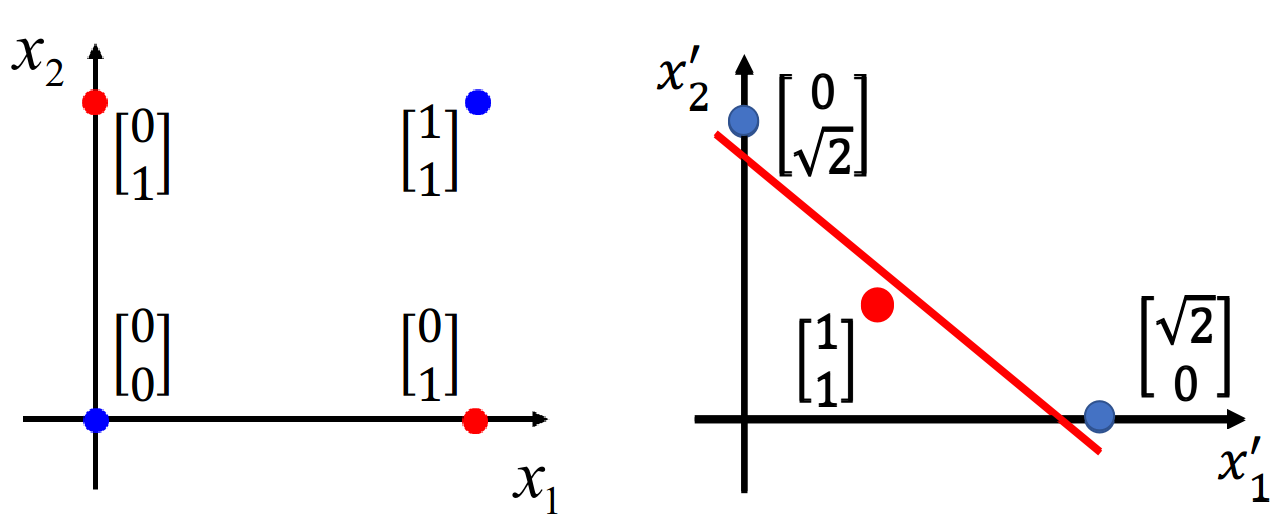
\includegraphics[width=0.6\linewidth]{transform.png}
    \caption{特征映射}
    \label{fig:transform}
\end{figure}

但实际上,如何做恰当feature Transformation本身就是个难题,如果在这上面花费太多时间就得不偿失了。\textbf{级联逻辑回归}的提出解决了这个问题,先用n个逻辑回归做特征转换,再用1个逻辑回归作为新特征的分类器,它们的参数都可以通过梯度下降来得到。

\subsubsection{级联逻辑回归到神经网络}
在级联逻辑回归中,如果把每一个逻辑回归叫做一个neuron(神经元),把这些用于feature Transformation的逻辑回归串联起来所形成的网络,叫做Neural Network(神经网络),那么级联逻辑回归就是我们所熟知的深度学习神经网络模型,sigmoid函数则是每个神经元的激活函数。

\begin{figure}[H]
    \centering
    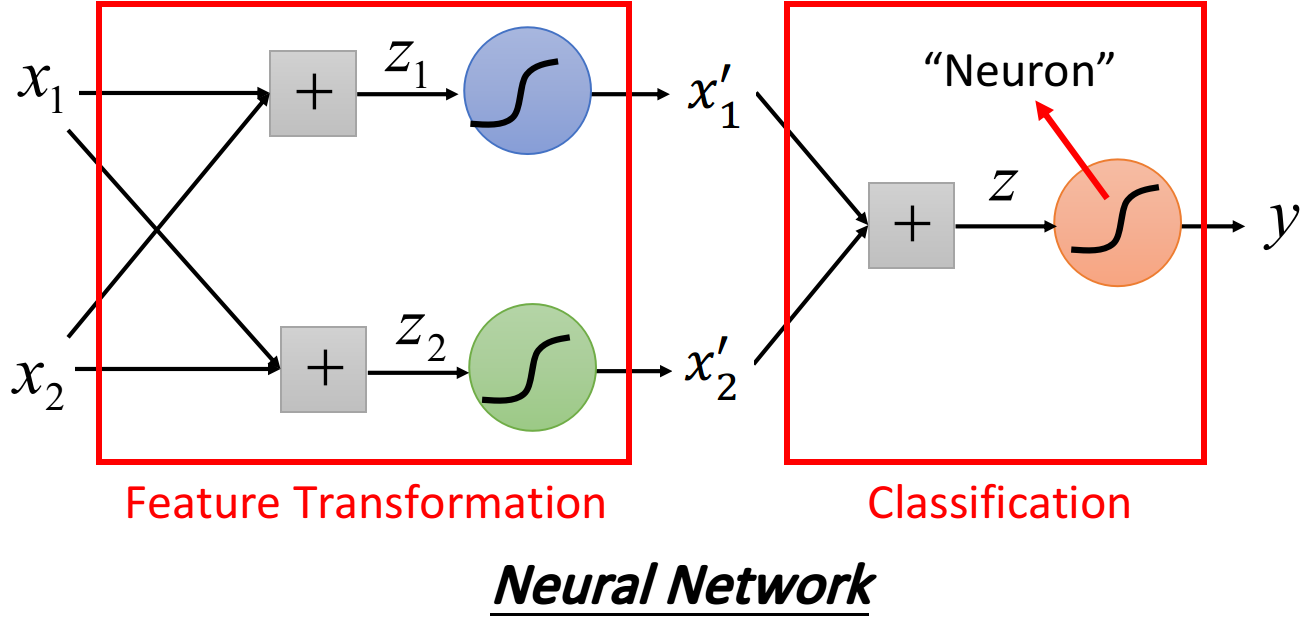
\includegraphics[width=0.8\linewidth]{nn.png}
    \caption{级联逻辑回归即神经网络模型}
    \label{fig:nn}
\end{figure}

\subsection{从神经网络到自编码器}
\subsubsection{神经网络的本质}
从前面的推导可以看出,神经网络的众多隐藏层本质上就是一个个特征提取器,随着网络层数的增加,检测的特征从简单变为复杂,最终通过后续的输出层分类器,得到分类的结果。\\

如果直接用神经网络作为分类器,也可以得到较好的分类效果。虽然神经网络的特征提取能力是毋庸置疑的,但在整个网络架构中,作为分类器部分的后几层layer并不一定能够得到充分的训练,导致分类准确率无法得到进一步的提升。\\

而本文的创新点在于,用随机森林、LightGBM等树模型作为神经网络后半部分的分类器。换一种说法就是,并不直接用神经网络作为分类器,而是\textbf{把神经网络提取到的特征用于训练其他更专业更高性能的分类模型}。实际操作上就是把神经网络隐藏层的输出接到其他分类模型的输入上,以期得到更好的分类效果。

\subsubsection{自编码器提取隐藏层输出}
如何获取隐藏层输出呢?自编码器(Auto-encoder)提供了一种很好的思路,它的基本思想是,通过神经网络将原先的高维特征投影到非线性的低维空间上,并通过同样的网络结构重新映射回原先的空间,利用还原前后样本特征之间的差异作为损失函数,直到可以实现稳定特征转换为止。

\begin{figure}[H]
    \centering
    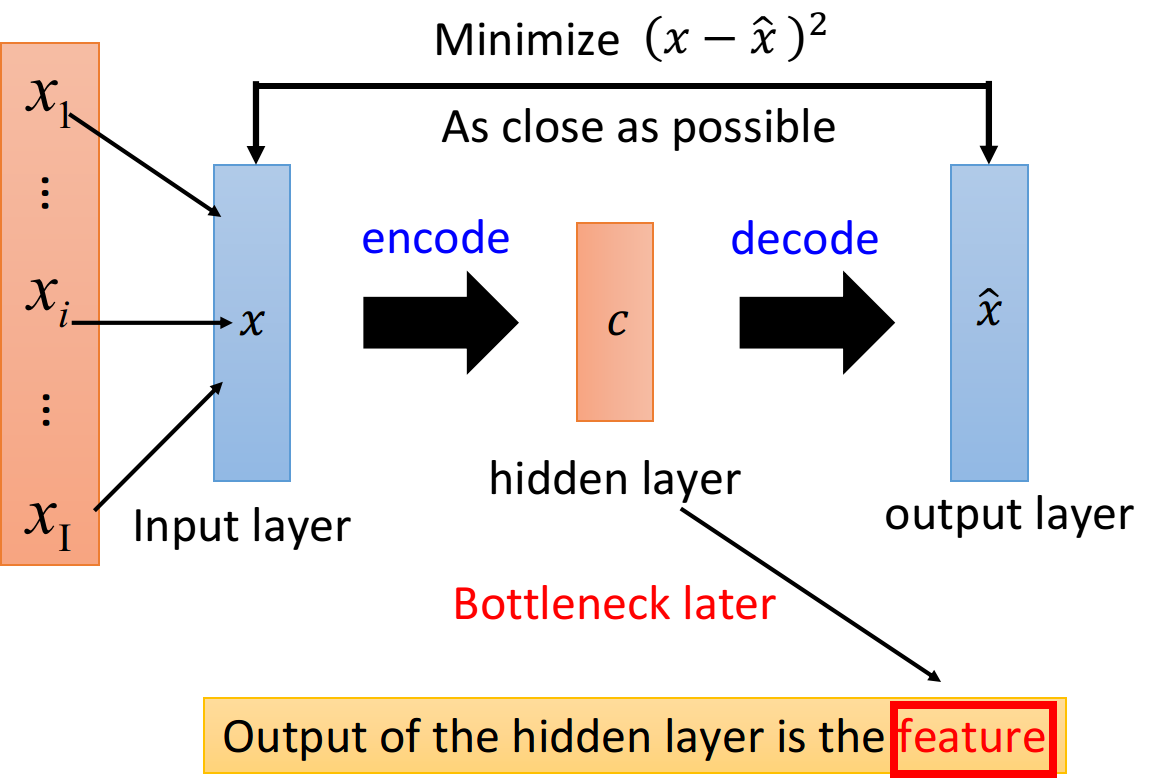
\includegraphics[width=0.6\linewidth]{autoencoder.png}
    \caption{自编码器提取特征}
    \label{fig:autoencoder}
\end{figure}

从图6中可以看出,中间hidden layer的输出就是我们希望通过神经网络提取到的特征,接下来用这些特征去训练随机森林、LightGBM等树模型,或是重新丢给一个神经网络分类器,来获取最终的分类结果。

\subsection{分类模型简介}
获取到新的特征之后,最终还是需要用专业的分类模型来划分样本点,本文主要使用随机森林、LightGBM、逻辑回归、DNN分类器来作为进一步的分类模型。这里将简要介绍随机森林和LightGBM这两个树模型。

\subsubsection{随机森林}
随机森林是一种集成算法(Ensemble Learning),它属于Bagging类型,通过组合多个弱分类器,最终结果通过投票或取均值,使得整体模型的结果具有较高的精确度和泛化性能。\\

Bagging也叫自举汇聚法(bootstrap aggregating),是一种在原始数据集上通过有放回抽样重新选出k个新数据集来训练分类器的集成技术。它使用训练出来的分类器的集合来对新样本进行分类,然后用多数投票或者对输出求均值的方法统计所有分类器的分类结果,结果最高的类别即为最终标签。此类算法可以有效降低bias,并能够降低variance。

\begin{figure}[H]
    \centering
    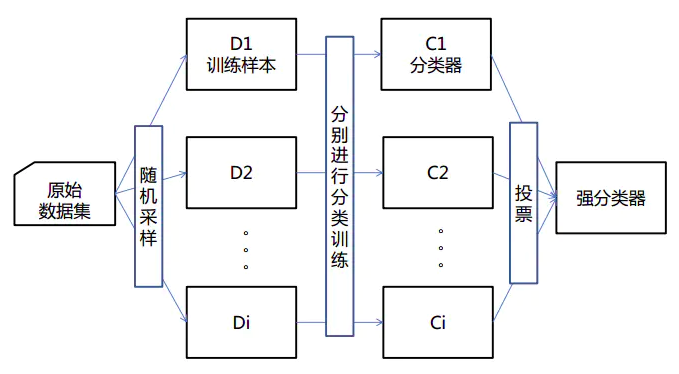
\includegraphics[width=0.6\linewidth]{rf.png}
    \caption{随机森林示意图}
    \label{fig:rf}
\end{figure}

随机森林的基本特性如下:
\begin{itemize}
    \item RF使用了CART决策树作为弱学习器
    \item 在生成每棵树的时候,每个树选取的特征都仅仅是随机选出的少数特征,一般默认取特征总数m的开方
    \item 相对于一般的Bagging算法,RF会选择采集和训练集样本数N一样个数的样本
    \item 由于随机性,对于降低模型的方差很有作用,故随机森林一般不需要额外做剪枝,即可以取得较好的泛化能力和抗过拟合能力
\end{itemize}

\subsubsection{LightGBM}
GBDT (Gradient Boosting Decision Tree) 是最常见的分类模型之一,其主要思想是利用弱分类器(决策树)迭代训练以得到最优模型,具有训练效果好、不易过拟合等优点。LightGBM (Light Gradient Boosting Machine)则是一个实现 GBDT 算法的框架,支持高效率的并行训练,并且具有以下优点:
\begin{itemize}
    \item 更快的训练速度
    \item 更低的内存消耗
    \item 更好的准确率
    \item 分布式支持,可以快速处理海量数据
\end{itemize}

GBDT在每一次迭代的时候,都需要遍历整个训练数据多次,导致训练效率低下,而LightGBM则针对这一情况做了优化,变得更轻量。它使用了基于 Histogram的决策树算法,根据直方图的离散值,遍历寻找最优的分割点。此外,它抛弃了大多数 GBDT 工具使用的按层生长 (level-wise) 的决策树生长策略,而使用了带有深度限制的按叶子生长 (leaf-wise) 算法。\\

Leaf-wise 是一种更为高效的策略,每次从当前所有叶子中,找到分裂增益最大的一个叶子,然后分裂,如此循环。同GDBT使用的 Level-wise 策略相比,在分裂次数相同的情况下,Leaf-wise 可以降低更多的误差,得到更好的精度。Leaf-wise 的缺点是可能会长出比较深的决策树,产生过拟合。因此 LightGBM 在 Leaf-wise 之上增加了一个最大深度的限制,在保证高效率的同时防止过拟合。\\

LightGBM 还具有支持高效并行的优点。LightGBM 原生支持并行学习,目前支持特征并行和数据并行的两种,并且针对这两种并行方法都做了优化。\\

